


%\titlerunninghead{Solar Control of Polar Irregularities}


%\authoraddr{L. J. Lamarche and R. A. Makarevich, Geophysical Institute, University of Alaska Fairbanks, 903 Koyukuk Drive, PO Box 757320, Fairbanks, AK, 99775-7320, USA.
%(rmakarevich@alaska.edu)}



%\linenumbers*[1]
%\begin{document}


\chapter{Solar control of \(F\) region radar backscatter: Further insights from observations in the southern polar cap}

%\authors{Leslie J. Lamarche\altaffilmark{1} and Roman A. Makarevich \altaffilmark{1}}
%\vspace{-1.5cm}


%\altaffiltext{1}{Geophysical Institute and Department of Physics, University of Alaska Fairbanks, Fairbanks, AK, USA.}



%\begin{abstract}

The role of solar wind and illumination in production of small-scale \(F\) region plasma irregularities is investigated using a 4-year data set collected by the Super Dual Auroral Radar Network (SuperDARN) facility at the McMurdo station, Antarctica (MCM). Statistical analysis of ionospheric echoes detected by MCM shows that radar backscatter from the polar \(F\) region occurs in wide and persistent bands in range that exhibit systematic changes with local time, season, and solar cycle. It is demonstrated that all variations considered together form a distinct pattern. A comparison with \(F\) region model densities and raytracing simulations shows that this pattern is largely controlled by the \(F\) region solar-produced ionization during the day. During the night, however, MCM observations reveal a significant additional source of plasma density in the polar cap as compared with the model. An example of conjugate radar observations is presented that supports the idea of polar patches being this additional source of ionization on the nightside. Echo occurrence exhibits a clear peak near the solar terminator, which suggests that small-scale irregularities form in turbulent cascade from large scales. Further, echo occurrence is enhanced for particular IMF orientations during the night. Observations indicate that solar illumination control of irregularity production is strong and not restricted to the nightside. Indirect solar wind control is also exerted by the IMF-dependent convection pattern, since the gradient-drift instability favors certain orientations between the plasma density gradients and convection velocity.

%\end{abstract}

%\begin{article}
\section{Introduction}
\label{Sec:Intro}

Plasma density waves or irregularities are commonly observed in both the \(E\) and \(F\) regions of the ionosphere and with scales ranging from a few centimeters to several kilometers. Several methods have been used to study ionospheric structures, including in situ rocket and satellite measurements as well as remote sensing using radio and optical techniques \citep{Fejer1980}.  In this study, we focus on small-scale irregularities (\(\sim\)10 m) in the \(F\) region that are thought to be primarily due to the gradient-drift instability (GDI) \citep{Tsunoda1988}.


Production of these irregularities is reasonably well understood on a microphysical level, with GDI promoting irregularity growth for certain orientations of the density gradient vector relative to the convection electric field \citep{Kesknien1982a,Kesknien1982b,Makarevich2014c}. The role of global factors, on the other hand, such as geomagnetic activity or solar wind conditions is much less investigated. In particular, the extent of the solar control is largely unknown, both in terms of its direct effects due to varying ionization and  indirect effects due to varying interplanetary magnetic field (IMF) as explained below. This is particularly important to processes occurring in the polar cap where some of the strongest differences in solar illumination conditions occur and where geomagnetic field lines are directly connected to the IMF.



One fundamental question under investigation in whether solar illumination suppresses or enhances irregularity production. In the auroral zone, evidence has been presented that solar illumination reduces the rate at which irregularities are observed by coherent radars in the Super Dual Auroral Radar Network (SuperDARN) \citep{Ruohoniemi1997,Koustov2004}.  This is thought to be due to the background electron density increasing and smoothing the density gradients required to drive GDI \citep{Ruohoniemi1997,Koustov2004}. Preliminary studies in the polar ionosphere, however, indicated that echo occurrence is much reduced during nighttime \citep{Bristow2011}, implying that either daytime echo occurrence is enhanced or nighttime occurrence is suppressed. This needs to be further investigated to determine why and how irregularity production in the polar region may differ from that in the auroral region.

Observations of decameter-scale irregularities with SuperDARN have an advantage of significant datasets accumulated under a wide variety of observational conditions. SuperDARN utilizes radio refraction in the High Frequency (HF) band to observe \(F\) region echoes or backscatter from decameter-scale irregularities when radar beam achieves orthogonality with local magnetic field (orthogonality condition). Because of importance of propagation conditions for HF radar observations, the echo occurrence rates observed by SuperDARN are taken as a lower limit of the irregularity occurrence rates \citep{Chisham2007}.


Several recent SuperDARN studies have found clear seasonal and diurnal trends in the \(F\) region echo occurrence that formed a distinct pattern which appeared to be qualitatively similar to that of the solar zenith angle (SZA) variations \citep{Kane2012,Ghezelbash2014a,Ghezelbash2014b}. However, it has been challenging to determine how occurrence explicitly depends on SZA for all seasonal and time sectors. The nighttime occurrence taken separately was demonstrated to be closely related to SZA-controlled \(F\) region density  variations \citep{Kane2012}, but no similarly-clear relationship has been demonstrated for datasets including daytime points.

One difficulty is the need to consider propagation effects of plasma density. These arise because of \(F\)-region density controlling the amount of refraction and either under- or over-refraction reducing echo occurrence when orthogonality condition is not met \citep{Milan1997,Danskin2002}. This is also related to how echo occurrence is generally considered a lower limit on irregularities (described above). There is some ambiguity about whether changing irregularity production or detection by the radar is most responsible for any observed trends.

The production/detection ambiguity issue can be addressed by considering how both occurrence and distance from the radar (slant range) change in responses to various factors \citep{Kane2012,Ghezelbash2014b}. This is because range variations are expected to be almost entirely due to propagation effects and the differences in responses are therefore mostly likely due to changing production. In order to claim production as the dominant source of occurrence variability, occurrence analysis must explicitly considers the echo location. In the current study this approach is employed to develop a comprehensive model of occurrence location, quantify echo location trends, and explicitly consider these trends when developing occurrence estimates. This is in contrast with previous studies that considered echoes detected in the entire (or fixed part) of the radar's field-of-view (FoV) \citep[e.g.][]{Kumar2011,Kane2012}.

In addition to direct effects of solar illumination, there is also interest in the indirect ways in which the Sun may control irregularity production in the ionosphere. It has been shown that negative IMF Bz generally leads to higher echo occurrence in the auroral \(F\) region \citep{Ballatore2001}. An even stronger IMF control has been demonstrated for the auroral \(E\) region irregularities \citep{Makarevich2012}. Some dependence on substorm phase (and hence indirectly on IMF) is also expected and has been observed \citep{Wild2008}. One way in which the IMF and echo occurrence variations may be related is through the IMF-controlled convection pattern \citep{Ruohoniemi1996,Pettigrew2010}. Convection changes lead to different orientations between convection velocity and density gradient vectors, which may, in turn, change GDI contribution to structuring processes \citep{Makarevich2014c}. The feasibility of this scenario is largely unknown and the extent of IMF control of polar cap echo occurrence is yet to be evaluated.

The overall aim of this study is to evaluate the extent of solar control on the production of \(F\)-region density irregularities in the polar cap ionosphere. Specifically, the objectives are to (1) quantify variations in \(F\) region backscatter location for different time sectors, seasons, and solar cycle phases, (2) analyze direct effects of solar illumination in irregularity production utilizing a comprehensive model of echo location, and (3)  establish the relationship between echo occurrence and IMF in the polar cap \(F\) region.


\section{Experiment Configuration and Data Processing}
\label{Sec:Exp}

The primary instrument used in this study is the SuperDARN McMurdo radar located at McMurdo Station, Antarctica (77.88\(\deg\) S, 166.73\(\deg\) E, geographic) \citep{Bristow2011}. Using a standard SuperDARN 3-letter radar code, this radar is referred to as MCM. SuperDARN is an array of coherent HF radars used to study processes in the Earth's ionosphere and magnetosphere. Radars are located at mid and high latitudes in both the Northern and Southern Hemispheres. Radars measure a 17-lag auto-correlation function (ACF) from which estimates of the Doppler velocity, power, and spectral width of ionospheric echoes in 75--100 range bins for each of the 16--24 radar beams are obtained. Each radar beam spans \(\sim3.25\deg\) horizontally and \(\sim30\deg\) vertically, with the entire FoV of \(\sim52\deg\)--\(78\deg\) in azimuth. Range bins typically start at 180 km and have a length of 15 km or 45 km and a radar scans through all beams in 60 s or 120 s depending on the mode of operation. Other details on operations and technical characteristics of SuperDARN radars are given by \citet{Chisham2007}.

The magnetic latitude (MLAT) of MCM is 80.0\(\deg\) S, based on altitude-adjusted corrected geomagnetic (AACGM) coordinate system with 2010 coefficients \citep[see recent paper by][]{Shepherd2014}. The MCM FoV covers the southern polar cap and beam 14 of MCM is most conjugate with beam 1 of the SuperDARN Rankin Inlet (RKN) radar that overlooks the northern polar cap. The current study focuses on MCM observations, but in order to facilitate future comparisons with conjugate observations, the data from beam 14 of MCM are considered. MCM has been in routine operations since February 2010 and the current study has considered the data from the first 4 years of operations 2010--2013.

Standard SuperDARN criteria were used to eliminate ground scatter (\(\left| V-\Delta V \right| <30\) m/s and \(\left| W-\Delta W \right| <35\) m/s), where \(V\) is the Doppler velocity, \(W\) is the spectral width, and \(\Delta V\) and \(\Delta W\) represent uncertainties in these quantities. In addition, measurements with SNR \(<\) 3 dB or \(W>\) 500 m/s were eliminated to reduce contribution from interference and other spurious echoes. In addition to standard operation modes, each SuperDARN radar has a set time periods where the radar is run in special modes. In order to have as continuous of a dataset as possible for the statistical analysis, data were used both from the standard modes and from special modes when possible. Modes where the beam 14 was over-sampled (beam camping modes) or not sampled at all were not used.

In this study, we also employed the IMF measurements taken from the high-resolution OMNI database using spacecraft-specific dataset for the WIND satellite. This was the OMNI dataset that had the largest number of valid measurements throughout the period of interest 2010--2013. All data in the OMNI database are time shifted from the spacecraft location to Earth's bow shock nose (BSN). The data were further shifted by 9--12 min to account for propagation from the BSN to the high-latitude ionosphere using a method described by \citet{Khan1999} that was also employed by \citet{Makarevich2012}. The IMF By and Bz components were averaged over 10-min intervals. Any periods with IMF information missing were excluded from the analysis.

The model electron densities were also used in the current study. The electron densities were found from the International Reference Ionosphere (IRI) 2007 model \citep{Bilitza2008}. The IRI model is an empirical model of the ionosphere based on time of day, date, geographic location, altitude, and solar conditions, with electron density near the \(E\) and \(F\) region peaks being of particular interest for this study.  Using ionosonde terminology, these are also referred to below as model NmE and NmF2.



\section{Observations}
\label{Sec:Obs}

In order to examine diurnal, seasonal, and solar cycle trends in echo occurrence, the monthly average occurrence was found for each universal time (UT) 2-min interval and for each 45-km range bin. If measurements were conducted at a 2-min resolution, each radar cell had an occurrence of 1 or 0. For a higher resolution, the values were weighted accordingly so that if an echo was observed for every possible time within the 2-min interval, the overall echo occurrence was still 1. The data for each time/range cell were averaged over the entire month. Figures \ref{fig:month_avg_occ}a--d show monthly average occurrence expressed in percentage for four selected months in year 2010 versus UT and slant range. The four months presented were chosen to be representative of different seasons. Figures \ref{fig:month_avg_occ}e--h on the right similarly shows the monthly average peak \(F\)-region electron density NmF2 obtained from the IRI model. The cosine white contours in both left and right panels show the approximate range position of the \(F\)-region echo band for each month determined as described below.
	
\begin{figure}
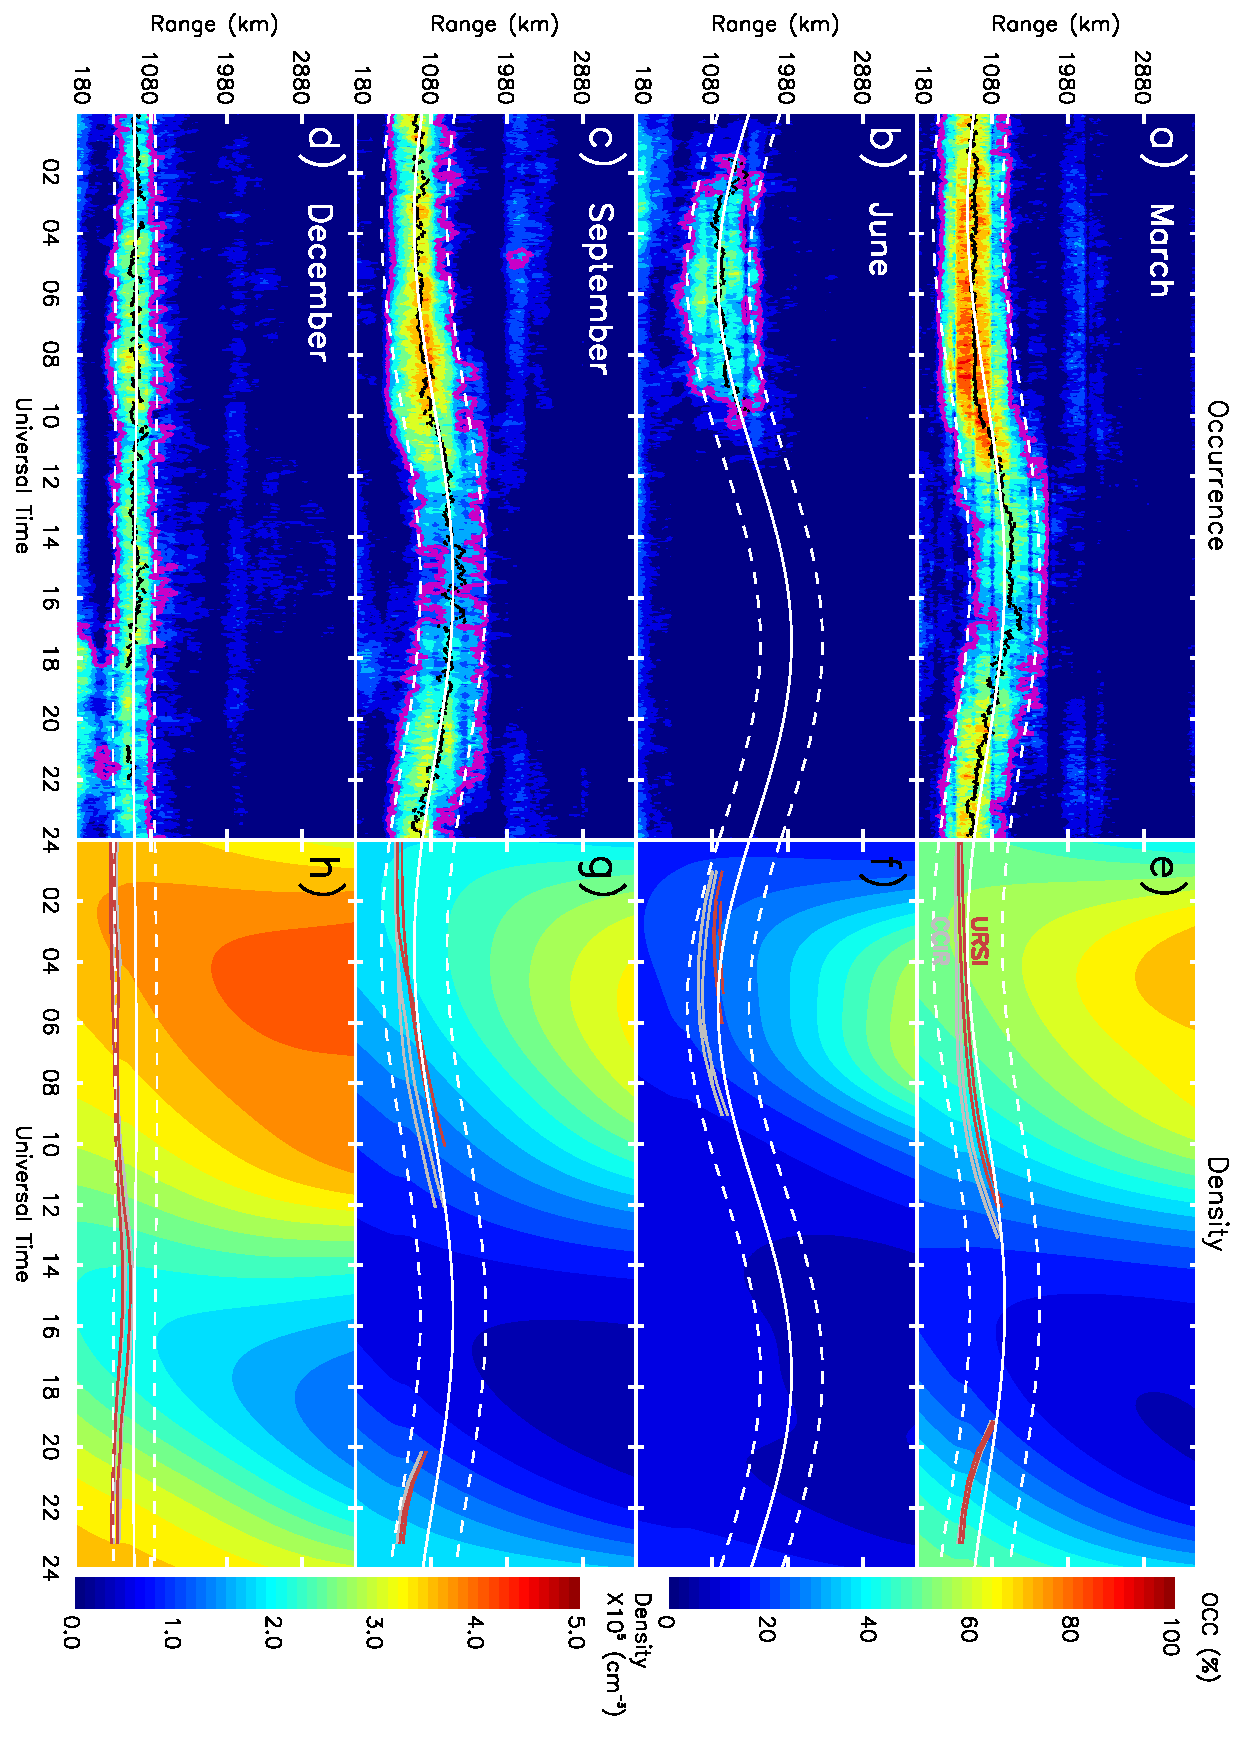
\includegraphics[width=12.5 cm,angle=90]{month_density_occurance2010.pdf}
\caption{Monthly average plots of echo occurrence (left) and peak electron density (right) for 2010.  Four months are selected (one for each season) to show seasonal variations. In Figures \ref{fig:month_avg_occ}a--\ref{fig:month_avg_occ}d,  the pink line shows the 25\% occurrence contour that is used to define the echo band region. Black dots are the midpoints between the upper and lower portion of this contour.  A cosine function (white line) is fit to these points and used to model the echo band. The dashed white lines are the upper and lower bounds of the model band. The top right corner of each panel shows the parameters that characterize the band for that month: \(A\) is amplitude of cosine function (in km), \(B\) is time shift (in hrs), \(C\) is range shift from 0 (in km), and BW is the band width (constant distance between the upper and lower dashed white lines).  In Figures \ref{fig:month_avg_occ}e--\ref{fig:month_avg_occ}h the same echo location model is also given (white lines) along with expected echo locations based on raytracing simulations (dark red line).}
\label{fig:month_avg_occ}
\end{figure}

Figures \ref{fig:month_avg_occ}a--d show a distinct \(F\)-region band of high occurrence in every month at ranges 500--1500 km. Some \(E\)-region echoes are also observed at shorter ranges 180--300 km in June at 01--06 UT and in December at 17--24 UT. The \(F\)-region band range position and peak occurrence within the band was changing most clearly throughout the day in March and September, i.e. diurnal variation in both parameters is observed clearly in spring and fall months. To highlight the high echo occurrence band, a contour of 25\% occurrence is plotted in each left panel by the pink line and this shows a clear diurnal, cosine-like variation with UT in March and September.

The midpoints were also found between the top and bottom parts of the pink 25\% occurrence contour and the cosine function of the form
\begin{equation}\label{E:Model}
R\left(t\right) = A \cos\left[2\pi\left(t-B\right)/24\right] + C
\end{equation}
was fitted to these points. Here \(R\) is the range of the center of the band in kilometers, \(t\) is the time in hours, and  \(A\), \(B\), and \(C\) are fit coefficients with units of kilometers, hours, and kilometers, respectively. The white solid line in each panel of Figure \ref{fig:month_avg_occ} shows the resulting fit \(R\left(t\right)\). The white dashed lines represent the upper and lower limits of the band.  They were calculated by first finding the average distance \(\sigma\) between points in the 25\% occurrence contour and the fitted cosine at the same time of day. The original cosine fit was then shifted up or down by this amount as \(R\left(t\right) \pm \sigma\) to give the upper and lower limits of the band.  These limits match the pink 25\% occurrence contour well because all the points in the pink contour are approximately the same distance away from the central fit (white solid line). The band width (BW) could then be defined as \(2\sigma\). The fit parameters and band width are given in the top-right corner of Figures \ref{fig:month_avg_occ}a--d. For the rest of this study, ``echoes within the band'' refer to data points that fall between the upper and lower white dashed lines. From Figures \ref{fig:month_avg_occ}a--d, both the center position and upper/lower bounds for the band shown by the white lines capture the band and its diurnal variation in range very well for all months. Therefore, these estimates are used below to quantify the echo band behavior, particularly in context of expected electron densities.

MCM is oriented in such a way that it samples daytime (nighttime) ionosphere in roughly the first (second) half of the day in UT. The electron density on the right of Figure \ref{fig:month_avg_occ} clearly shows higher daytime densities that reach a peak near 05 UT at farther ranges and lower nighttime densities that reach a minimum near 17 UT. The \(F\)-region echo band thus was closer to the radar in the daytime (high densities) and farther away at night (low densities). This feature is most clear for the March and September datasets. It is much less clear in June, although one can still see a portion of the cosine-like variation at 02--10 UT in June in the pink contour. In this month, the white contours are mostly extrapolation outside of this interval, but they fit into the overall diurnal/seasonal pattern well (see also next analysis).  In December, the band is flat and diurnal variation is not evident.

In terms of diurnal variation of echo occurrence, there was a minimum occurrence at nighttime and a maximum in daytime hours. The minimum was much deeper and more extended in June so that essentially no echoes were observed at 12--24 UT. At this time, the expected location of echoes based on the cosine-fit model (white lines) is farther away from MCM than in any month and any UT interval, but no echoes are observed either at these ranges or any other ranges. This is in contrast with March and September, where occurrence is reduced at nighttime but not to zero. Overall, Figure \ref{fig:month_avg_occ} shows that range position of the band is largely controlled by the density conditions, while the echo occurrence variation is perhaps more complicated.

The final observation about Figure \ref{fig:month_avg_occ} concerns the results of raytracing simulations that were conducted for each hour of day 15 in each of the four months shown in Figure \ref{fig:month_avg_occ}. In these simulations, IRI densities in a 2D simulation domain aligned with beam 14 of MCM were used. The range locations where orthogonality condition was expected are plotted in Figures \ref{fig:month_avg_occ}e--h by the dark red line. The gaps during the nighttime in these lines in all months but December indicate that no orthogonality was expected at any range in MCM beam 14 during these periods. The red line is located between the solid and bottom dashed white lines, indicating a reasonable agreement between the expected and observed backscatter locations. The important exception is seen, however, for nighttime periods (or, more accurately, whenever densities were lower than \(\sim1.5\times10^5\) cm\(^{-3}\), dark blue colors). During those periods, no orthogonality was expected based on IRI densities, but significant (albeit reduced) amount of backscatter was observed in March and September. This implies a significant source of nighttime plasma density that is unaccounted for by the IRI model.



The same analysis was performed for the entire period of interest 2010--2013 and the band characteristics are presented in Figure \ref{fig:year_line}. It shows the band (a) position amplitude \(A\), (b) time shift \(B\), (c) range position \(C\), and (d) width (BW) plotted versus month.  Each year is shown as a line in a different color as indicated in the top-right corner of panel (a).

\begin{figure}
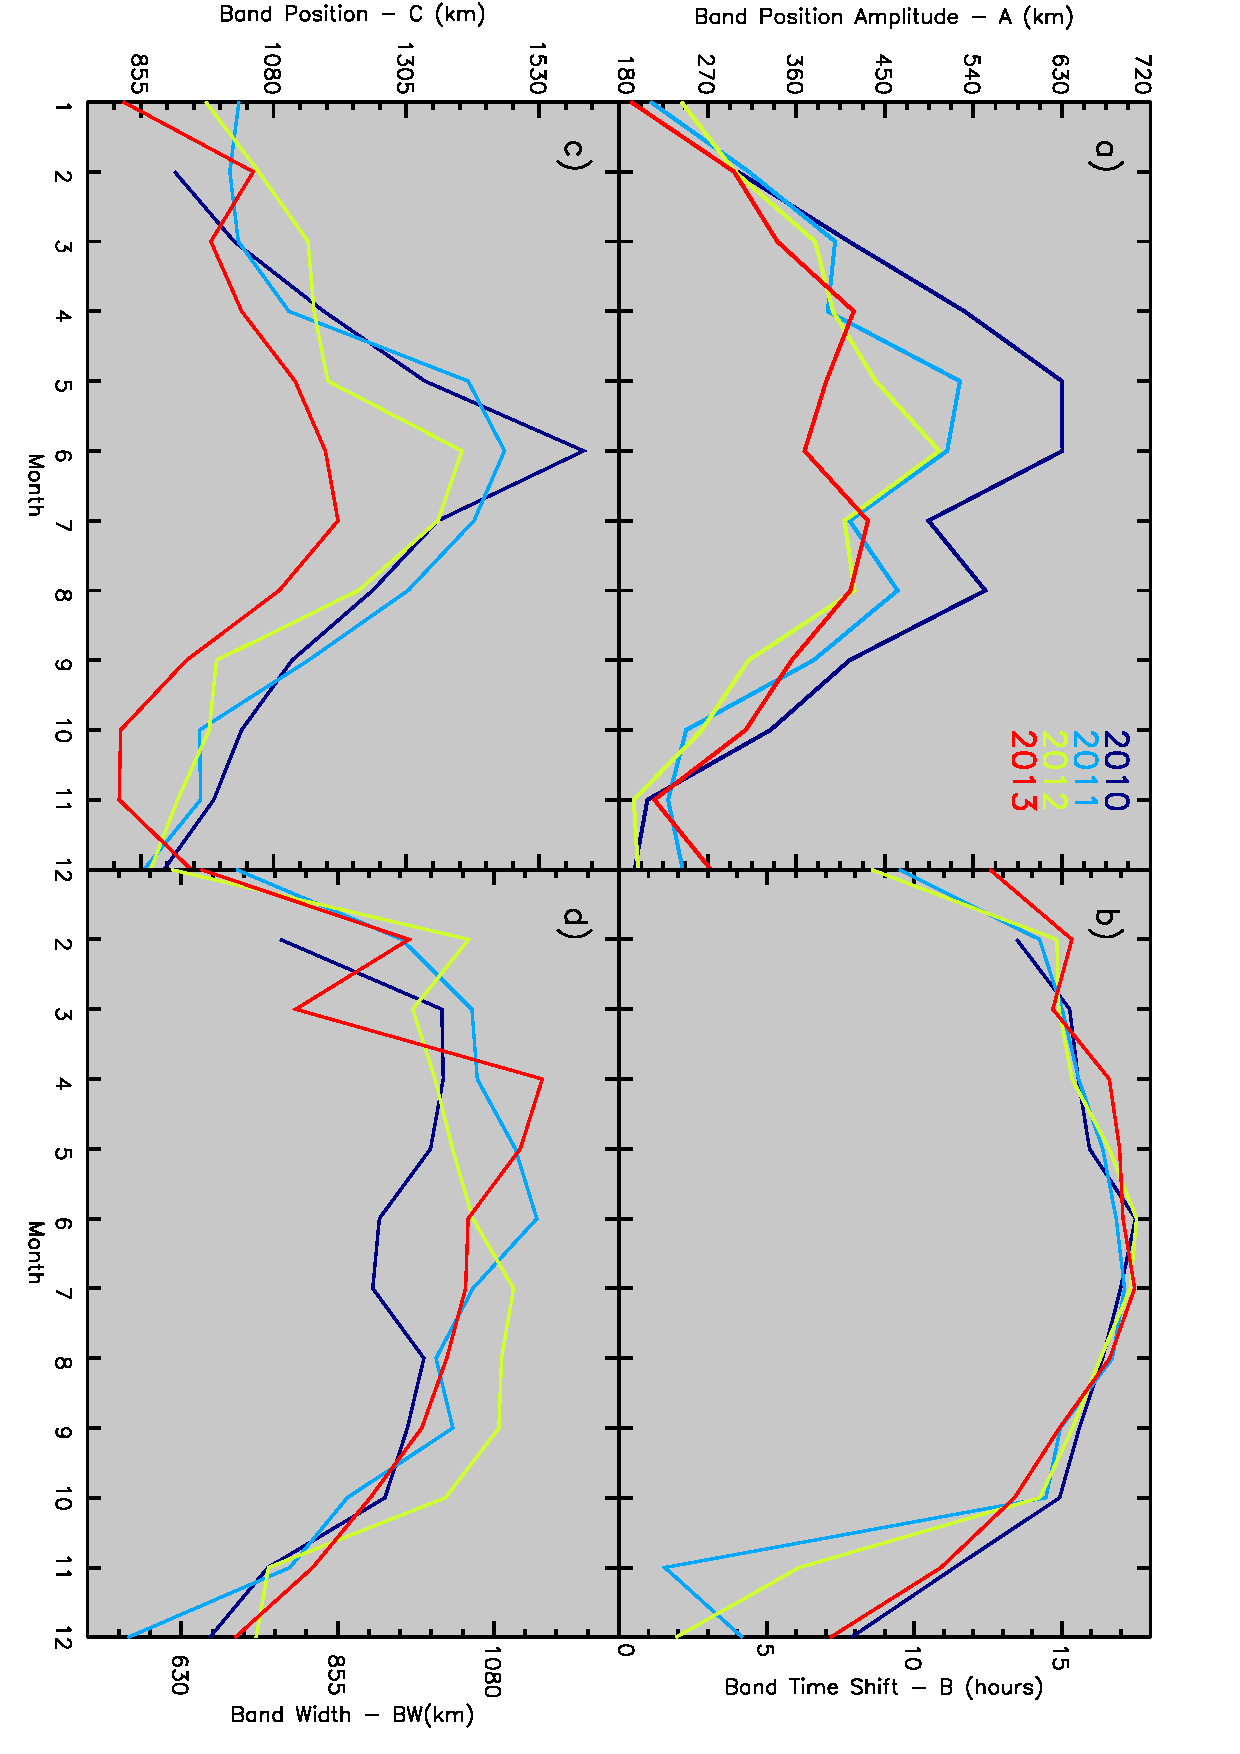
\includegraphics[width=11.0 cm,angle=90]{year_month_analysis_line.pdf}
\caption{The variations in the echo band (a) amplitude of the fitted cosine function \(A\), (b) time shift or time of day of the peak \(B\), (c) average position of the band or the vertical shift of the cosine function from zero \(C\), and (d) width (BW). Different lines are for different years with the legend given in Figure \ref{fig:year_line}a.}
\label{fig:year_line}
\end{figure}

All four parameters peak in austral winter and decrease in summer months. Solar cycle variation is evident in (a) the band position amplitude and (c) the average band position. In general, both parameters were larger in years closer to solar minimum (year 2010) and decreased moving towards solar maximum (2013).  In both cases, the variation existed primarily in the winter months (around June). In contrast, the seasonal variation was also evident in (b) the band time shift and (d) the band width, but no clear solar cycle trend was present. In fact, the band time shift was quite consistent between different years, except for winter months. This parameter was typically around 15 hrs. This is when a maximum of \(R\left(t\right)\) was observed in UT, i.e. when band position was located furthest away from the radar.

In the previous analysis, the focus was on band characteristics related to range and their variations. The next presentation examines the diurnal/seasonal/solar cycle pattern as a whole for both band range position and one other important characteristic, the echo occurrence within the band. For each month, the band position \(R\left(t\right)\) and the average occurrence between \(R\left(t\right)\pm \sigma\) were found similar to those presented in Figure \ref{fig:month_avg_occ}. A horizontal slice of each panel of Figure \ref{fig:year_color} represents the time series for one month. The band position \(R\left(t\right)\) (average echo occurrence) is shown in Figures \ref{fig:year_color}a--\ref{fig:year_color}d (Figures \ref{fig:year_color}e--\ref{fig:year_color}h) as a color contour plot representing the time series for all months of the year simultaneously; different rows refer to  different years. The left panels look much smoother than the right ones; this is simply because each line on the left is a fitted cosine \(R\left(t\right)\), while on the right it is the average ``raw'' occurrence between two fitted cosine lines \(R\left(t\right)\pm \sigma\). The white data gaps at the bottom of Figures \ref{fig:year_color}d and \ref{fig:year_color}h reflect the fact that no MCM data were collected in January 2010.
	
\begin{figure}
\includegraphics[width=12.0 cm,angle=90]{year_month_analysis_color.pdf}
\caption{Contour plots of the (a)--(d) echo band range and (e)--(h) occurrence versus UT and season. Each row shows the data for a different year as given in the top-right corner.}
\label{fig:year_color}
\end{figure}

In Figures \ref{fig:year_color}a--d, the band position \(R\left(t\right)\) peaks in nighttime (second half of the day) and in winter. This peak (yellow-to-red colors) is seen in the same plot area as the low occurrence plot cells in Figure \ref{fig:year_color}e--h (blue color). The amplitude of the range peak became consistently lower between 2010--2013.  This indicates that the high occurrence band moved closer to the radar for years further away from the solar minimum.

The minima in the band position \(R\left(t\right)\) (blue contours) were observed during the daytime and near equinoxes. This feature was most clear in 2010 when these minima were observed near 03 UT in March and September; these were also the two months presented in Figure \ref{fig:month_avg_occ}. The echo occurrence pattern, Figures \ref{fig:year_color}e--h, is less clear in terms of its maxima and their relationship with range minima. Typically, one equinoctial maximum was more pronounced as in 2011--2013, with no clear preference towards either March of September. In 2010, the two maxima are most similar (yellow contours), but the UT peak was shifted away from that of the range minimum (by about 5 hours). Overall, however, the range and occurrence patterns appear to be inverse of each other: larger range means smaller occurrence and vice versa.

The diurnal, seasonal, and solar-cycle variations in echo occurrence observed in Figures \ref{fig:month_avg_occ}--\ref{fig:year_color} can be explained by looking at the solar zenith angle (SZA) and ionospheric density conditions. SZA indicates how sunlit the ionosphere is and the associated degree of ionization, i.e. the \(E\)- and \(F\)-region electron densities, as explained in Section \ref{Sec:Intro}. The model NmE and NmF2 values have been employed for this analysis, Section \ref{Sec:Exp}. To keep model run times at a manageable level, here we consider 10-min cadence data including the average echo occurrence within the band (in Figures \ref{fig:month_avg_occ}--\ref{fig:year_color}, the 2-min data were considered).



Figures \ref{fig:scatter}a and \ref{fig:scatter}b present the results of this analysis for year 2010 in the form of scatter plots of band position versus (a) SZA and (b) model NmF2, while Figures \ref{fig:scatter}c and \ref{fig:scatter}d are scatter plots of echo occurrence versus (c) SZA and (d) model NmF2. In all four panels, the model NmE is shown by the color of the points, with the color bar given to the right. The points in the top row show some clustering in the form of closed loops (some of them appear just as horizontal lines). This is simply a consequence of the periodic nature of the cosine fit; each loop refers to the data for one month. The summer months exhibit little-to-no variation; these appear as horizontal loops-lines.

\begin{figure}
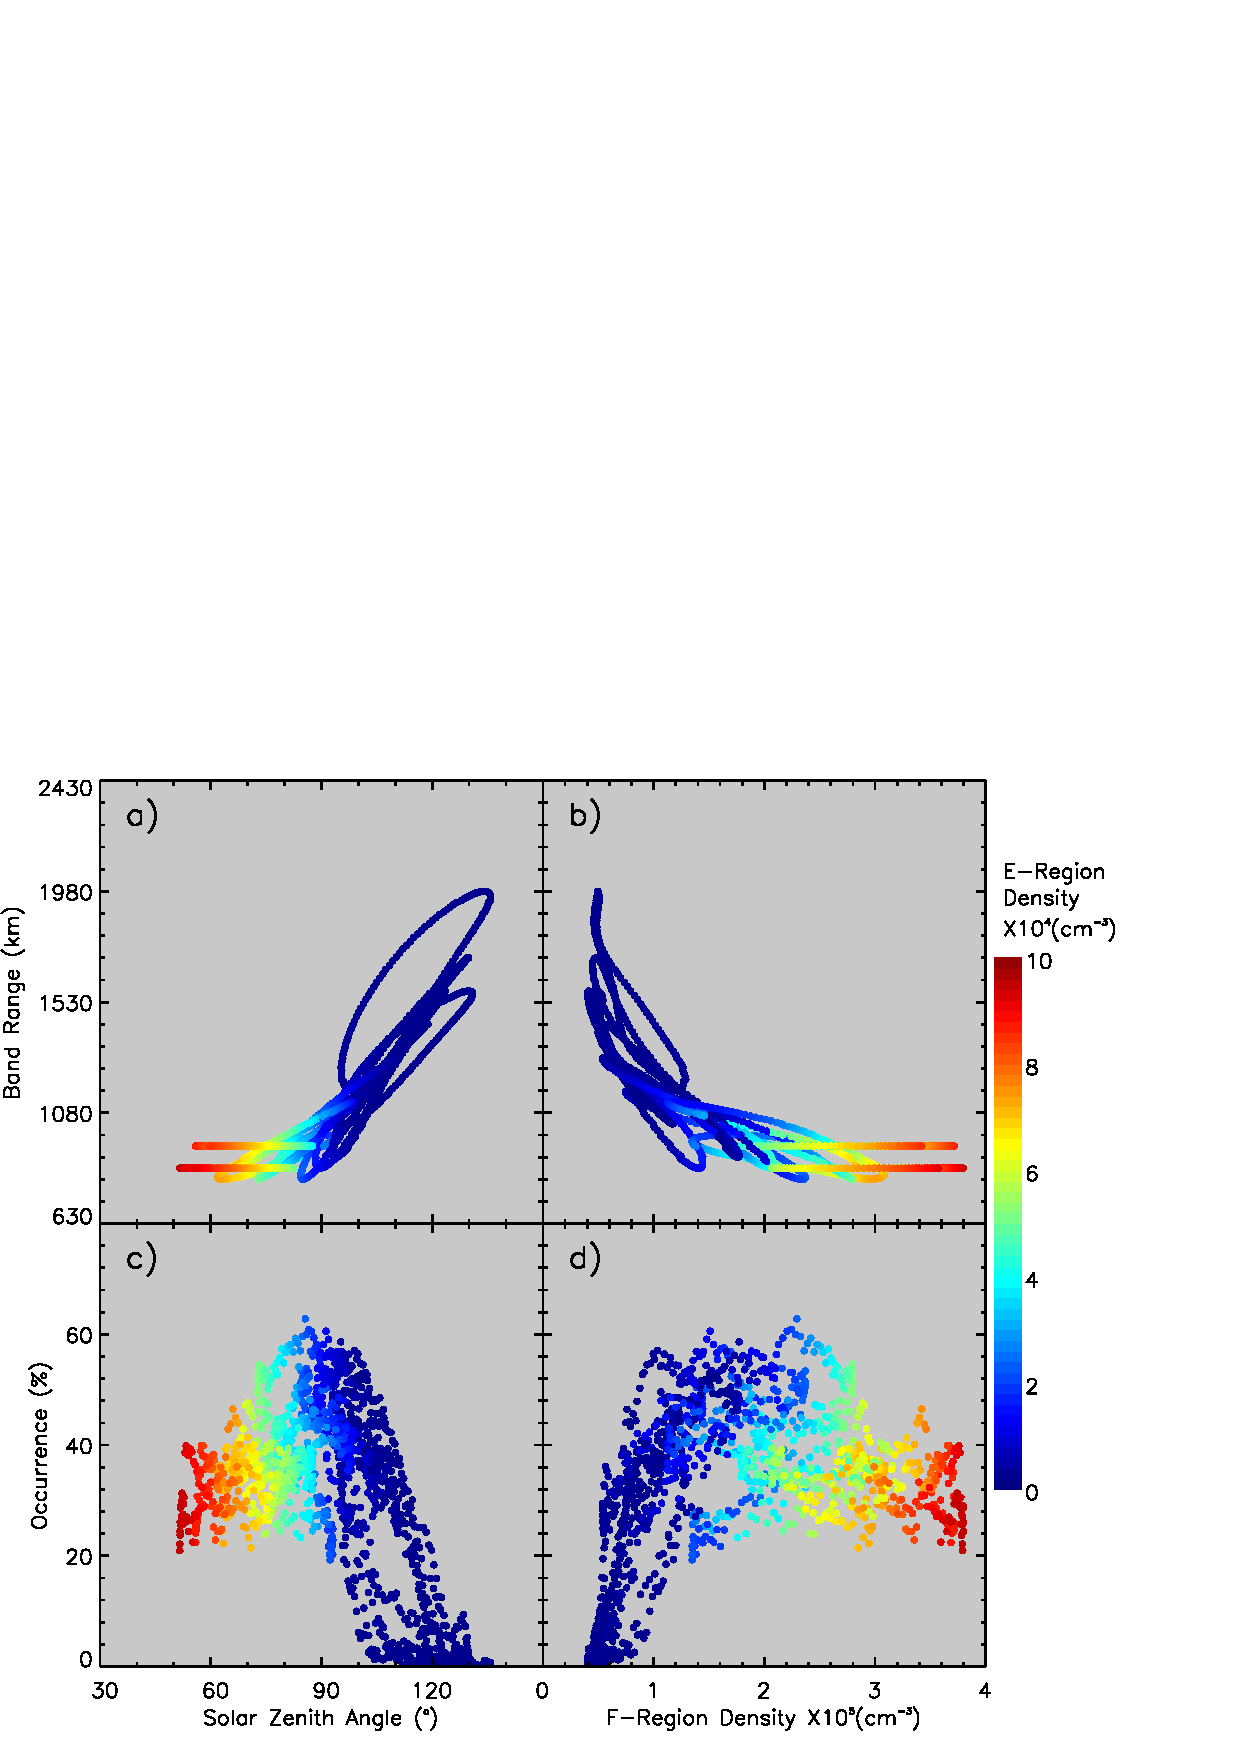
\includegraphics[width=17.0 cm]{scatter_E2010.pdf}
\caption{The echo band range versus the (a) solar zenith angle (SZA) and (b) model peak F2 electron density (NmF2). Each point is color-coded in model \(E\) region density. Figures \ref{fig:scatter}c and d show the same but for the  echo occurrence within the band.}
\label{fig:scatter}
\end{figure}

Figure \ref{fig:scatter}a shows a group of blue points referring to nighttime observations (SZA \(>\) 90\(\deg\)) that slope upwards from a band position range of \(\sim\)800 km to \(\sim\)2000 km with a SZA increasing. This indicates that the band moved into further ranges as radar sampled sectors farther away from sunset. The color of the points indicates that \(E\)-region electron density was typically lower at these times as well, as expected. In Figure \ref{fig:scatter}b, the same trend is seen as blue points starting at intermediate NmF2 values of \(\sim1.5 \times 10^5\) cm\(^{-3}\) and low ranges near 800 km, but increasing to ranges of \(\sim\)2000 km as NmF2 decreased to low values of \(\sim0.5 \times 10^5\) cm\(^{-3}\). This indicates that both representations (using SZA or model NmF2) are approximately equivalent: the band was further from the radar at low NmF2/high SZA values. At high NmF2/high NmE/low SZA values, i.e. during daytime conditions, the range did not change much. In summer months (horizontal loops mentioned above) in particular, this variation was virtually nonexistent. Overall, Figures \ref{fig:scatter}a and \ref{fig:scatter}b show a clearly-defined pattern of a decreasing band position \(R\left(t\right)\) with \(t\) moving away from sunset and SZA increasing from 90\(\deg\), NmF2 decreasing and NmE also decreasing.

The echo occurrence within the band shows a different pattern, Figures \ref{fig:scatter}c and \ref{fig:scatter}d. Occurrence increases towards SZA \(\approx90\deg\) during daytime, but then starts to decrease away from this value (Figure \ref{fig:scatter}c). The $E$-region density, on the other hand, appears to decrease monotonically with a SZA increasing. It has a peak at \(10 \times 10^4\) cm\(^{-3}\) at the smallest possible values of SZA \(\sim50\deg\), while occurrence peaks around 90\(\deg\). This means that echoes are most likely to be observed close to the terminator. There appears to be a similar peak when occurrence is plotted against \(F\)-region electron density (Figure \ref{fig:scatter}d). The NmF2 value corresponding to occurrence peak is between \(1.0\times 10^5\)--\(2.5\times 10^5\) cm\(^{-3}\) depending on the month.  At both lower and higher \(F\)-region densities, occurrence decreases. This indicates that there is a range \(F\)-region electron densities that favors the observation of echoes. In both Figures \ref{fig:scatter}c and \ref{fig:scatter}d, points where the \(E\)-region density is high (dark red points) have relatively low occurrence.  Based on Figure \ref{fig:scatter}c, these generally have the lowest occurrence of all daytime measurements.  Overall, Figures \ref{fig:scatter}c and \ref{fig:scatter}d show that echo occurrence peaks near the terminator where NmF2 is moderate and decreases for SZA increasing and decreasing from 90\(\deg\).

The IMF variations have been previously shown to affect HF radar observations of the auroral ionosphere in both the \(F\) region \citep{Ballatore2001} and \(E\) region \citep{Makarevich2012}. The IMF variations are a consequence of solar activity and are not related to the time of day or season, so they must be studied independently. IMF activity is also related to solar cycle, but the correlation is on a time scale of about a decade. In the following analysis, we attempt to determine whether there is a direct relationship between IMF behavior and echo occurrence on the scale of a few hours. We compare the MCM echo occurrence variations with the simultaneous IMF observations using a method analogous to that employed by \citet{Makarevich2012} in their study of auroral \(E\)-region irregularities (see also our section \ref{Sec:Exp} for a brief description of IMF data analysis).

The average occurrence within the band was found at 10-min intervals as in the previous analysis. The average IMF components over corresponding 10-min intervals were also found. Figure \ref{fig:ut_occ} presents the entire 4-year dataset of echo occurrence versus UT, with color representing average IMF component over each plot bin. The bin sizes were 1-h in time and 2\% in occurrence and Figure \ref{fig:ut_occ} shows contour plots made using this grid. The color bar for all three IMF components is shown to the right.

\begin{figure}
\includegraphics[width=15.0 cm]{IMF_vs_occ_MLT_avg.pdf}
\caption{IMF effects in echo occurrence. The echo occurrence versus UT was binned in 1-hr bins in UT and 2\% bins in occurrence and the average IMF (a) Bx, (b) By, and (c) Bz components over each plot cell are shown by the color.}
\label{fig:ut_occ}
\end{figure}

Figure \ref{fig:ut_occ}a and \ref{fig:ut_occ}c show minimal color structure in the first half of the day (0--12 UT; daytime observations). This indicates that in this time sector, neither positive nor negative IMF Bx or Bz was conducive to high echo occurrence. The dark blue region between 20\%--60\% occurrence and 0--10 UT of Figure \ref{fig:ut_occ}b (By component) indicates some association between low occurrence and negative By. The second half of the day (12--24; nighttime observations) exhibits a definite color structure for all three IMF components. Figure \ref{fig:ut_occ}a has an orange and yellow area between 18--21 UT at above 60\% occurrence. This means that in this time sector, high echo occurrence was observed during predominantly positive IMF Bx. Similarly, in Figure \ref{fig:ut_occ}b, the large blue area between 12--24 UT and above 50\% indicates an association between high occurrence and negative IMF By. Moreover, Figure \ref{fig:ut_occ}b shows that the color changes roughly monotonically from orange and yellow to green and blue with increasing occurrence. This means that higher occurrence was observed for more negative IMF By. A similar color structure is less clear in Figure \ref{fig:ut_occ}c (Bz  component), but still present. For example, Figure \ref{fig:ut_occ}c has a blue section above 70\% occurrence and between 16--24 UT, so high occurrence is also associated with negative IMF Bz in this sector. A similar change in color (from yellow to blue) with an increase in occurrence is also observed here, although it is not as monotonic (color pattern is somewhat patchy). Overall, this analysis indicates that higher nighttime occurrence is seen during periods of more positive Bx, negative By, and negative Bz.

Figure \ref{fig:by_bz} contains the same IMF data as Figure \ref{fig:ut_occ}, but here the IMF By and Bz effects are compared directly. IMF By and Bz are plotted on the horizontal and vertical axes, respectively, and color indicates relative occurrence, which was found as explained below. First, the average echo occurrence within the band over the whole month was found at 10-min intervals (these values were previously presented in Figure \ref{fig:year_color}, but at 2-min resolution). This time series was then subtracted from the average echo occurrence within the band for each day of the month (no averaging over the month). This resulted in a time series that approximately represents the variation in echo occurrence relative to a quiet-day season-specific diurnal average or the relative occurrence. This approach allows us to isolate the IMF effects from those due to diurnal and seasonal variations \citep{Makarevich2012}. Points were divided into six groups based on UT and plotted in different panels of Figure \ref{fig:by_bz}.

\begin{figure}
\includegraphics[width=11.0 cm,angle=90]{occ_vs_IMF_avg.pdf}
\caption{Relative occurrence versus IMF By and Bz components for 6 different UT sectors. Each plot cell is color-coded based on the average relative occurrence over that cell.}
\label{fig:by_bz}
\end{figure}

Figures \ref{fig:by_bz}a--\ref{fig:by_bz}c (representing 0--12 UT) show very little color structure.  Each panel is uniformly patchy, indicating no preference towards relatively high or relatively low echo occurrence for any IMF conditions. This is consistent with the minimal color structure observed in the 0--12 UT interval in Figure \ref{fig:ut_occ}. In the second half of the day (Figure \ref{fig:by_bz}d--\ref{fig:by_bz}f), the left half of each panel is more red and orange, while the right half is more blue. In particular, Figure \ref{fig:by_bz}d has a peak in relative occurrence (orange) at (\(-3, -2\)) nT in the (By, Bz) coordinates and an occurrence trough (blue) at (\(+5, -3\)) nT. Figure \ref{fig:by_bz}e has a region of high relative occurrence between (\(-\)4--0, \(-\)8--0) nT and a region of low relative occurrence between 2--10 nT in IMF By.  Figure \ref{fig:by_bz}f generally has high relative occurrence in the bottom-left corner of the panel and low relative occurrence in the top-right corner of the panel. This means that high (low) relative occurrence is observed for periods of negative (positive) IMF By and Bz. Comparing Figures \ref{fig:by_bz}d--\ref{fig:by_bz}f, the dividing line between the red/orange areas and the blue area is close to vertical in Figure \ref{fig:by_bz}e (along By \(\sim\)0 nT), but rotates to be at almost 135\(\deg\) in Figure \ref{fig:by_bz}f (stretching between the top-left and bottom-right corners). Overall, these results indicate increasing importance of the Bz component in the last time sector, namely, positive Bz leads to negative relative occurrence. These results also agree with those shown in Figure \ref{fig:ut_occ}, where the patch of blue (negative Bz) was seen between 16--24 UT and above 70\% occurrence.



\section{Discussion}

In this study, a comprehensive data set collected by the SuperDARN McMurdo radar over 4 years has been employed to investigate formation of small-scale irregularities in the polar \(F\) region, with a particular focus on global factors. MCM routinely observes backscatter from ionospheric irregularities over extended time periods and large spatial areas within the southern polar cap (``persistent backscatter''), which allowed us to reliably quantify both backscatter location and occurrence characteristics and investigate their control by the solar wind and illumination. By considering both location and occurrence we achieved better understanding and differentiation between radio- and plasma-physical factors or, alternatively, between irregularity detection and production. Below we further discuss three groups of issues aligned with three objectives of this study.

\subsection{\(F\) Region Echo Band: A Comprehensive Model and Density Implications}

Previous investigations of small-scale irregularity formation in the polar cap \(F\) region have primarily used SuperDARN coherent radars in both northern and southern polar caps \citep{Bristow2011,Ghezelbash2014b,Koustov2014}. These observations revealed unusually high echo occurrence rates of \(F\) region backscatter that can exceeded 80\% \citep{Bristow2011,Ghezelbash2014b}. These polar cap occurrence rates significantly exceed similarly-derived occurrence rates at auroral latitudes where the highest reported values were near 60\% under much stronger solar activity conditions \citep[e.g.][]{Koustov2004}.

One possible reason for this difference is more favorable propagation conditions in the polar cap with greater chances to reach orthogonality with magnetic field, which is a necessary condition for Bragg scatter to be received by coherent scatter radars. Whether any observed occurrence trend is due to changing propagation or production is difficult to resolve based on HF radar echo occurrence observations alone, as explained in section \ref{Sec:Intro}. A reasonable assumption often utilized is that propagation will be mostly responsible for changing location of echo occurrence. Typically, the entire FoV (or its large portion) is considered in calculating occurrence rates and, assuming range variations stay within the FoV, occurrence variability will be mostly due to changing production \citep[e.g.][]{Kane2010}. A considerable improvement over this approach is to explicitly consider the trends in backscatter location as well \citep{Kane2012,Ghezelbash2014b}. This way, any variation in occurrence and location is most likely due to a production factor. The current study refines this approach by including the location information explicitly in the way occurrence estimates are obtained. Further, the information about variations in the typical ranges of backscatter is important by itself, particularly since it directly reflects variations in the \(F\) region density. This provides a useful (albeit somewhat indirect) way to monitor and analyze plasma production and transport processes in a region where few opportunities for direct continuous measurements of plasma density currently exist.


The two important outcomes of the current study related to this indirect density analysis were (1) development of an empirical model to describe location of \(F\) region backscatter and (2) analysis of characteristics derived from the model. The \(F\) region backscatter was predominantly observed in the form of a band that was well described by a simple model, equation (\ref{E:Model}). The \(F\) region echo band exhibited systematic diurnal and seasonal effects, Figure \ref{fig:month_avg_occ}, which was reflected in systematic changes of the fitted band characteristics \(A\), \(B\), \(C\), and band width (BW), Figure \ref{fig:year_line}. These changes were quite consistent with those expected for plasma density. For example, the echo band was moving to further ranges during the night while density expected from IRI model was decreasing, Figures \ref{fig:month_avg_occ}e--h. Similarly, the amplitude of range variations \(A\) and average position \(C\) of the echo band exhibited seasonal and solar cycle variations consistent with those expected for densities, Figures \ref{fig:year_line}a and c.

Another novel aspect of the current study was a comprehensive set of raytracing simulations that was conducted using IRI densities. In general, the diurnal and seasonal variations were very similar between simulations (red line in Figures \ref{fig:month_avg_occ}e--h) and observations (white lines). One important exception was observed during the night near equinoxes. No orthogonality was predicted by model simulations, whereas a significant (albeit reduced) amount of backscatter was observed, Figures \ref{fig:month_avg_occ}a and c. That is, an occurrence gap (i.e. no backscatter) similar to what was observed in austral winter (Figure \ref{fig:month_avg_occ}b) was expected but not observed.



This result is significant as it implies a considerable additional source of density which would provide additional refraction and bring backscatter to orthogonality at the ranges consistent with the model. This prompts an important question about the origin of this source. It is unlikely that it was local since this production is well described by IRI \citep[e.g.][]{Themens2014}. A reasonable assumption is then that additional density was transported from somewhere else. The two phenomena that can be responsible for this are polar patches \citep{Weber1984} and sun-aligned arcs \citep{Valladares1994}. The polar patches in particular are known to travel long distances across the polar cap and even well into the nightside auroral zone \citep{Moen2007,Oksavik2010}.

Direct density measurements are not available near MCM but more insights can be obtained from observations in the conjugate northern polar cap. Figure \ref{fig:patchy_example} shows an example of conjugate measurements during two selected events that fall within the equinoctial period of Figure \ref{fig:month_avg_occ}a. Shown are (a) IMF By and Bz components, (b) MCM line-of-sight velocity in beam 14 versus UT and range, (c) RKN velocity in nominally-conjugate beam 4, and (d) northern face of the Resolute Bay incoherent scatter radar (RISR-N) measurements of electron density versus UT and altitude on March 14, 2010. Figures \ref{fig:patchy_example}e--h present the same information but for a second event on April 6, 2010.

\begin{figure}
\includegraphics[width=18.0 cm]{Fig_RISR.pdf}
\caption{Conjugate measurements for two selected events on (left) March 14, 2010 and (right) April 6, 2010. Shown are the (a) and (e) IMF By (blue) and Bz (red) components, (b) and (f) MCM line-of-sight velocity versus UT and slant range in beam 14, (c) and (g) RKN velocity in beam 4, and (d) and (h) RISR-N electron density versus UT and altitude. The color bar is the same for the two middle rows and is given to the right of Figure \ref{fig:patchy_example}f.}
\label{fig:patchy_example}
\end{figure}

Figure \ref{fig:patchy_example}b shows an echo band that fits well with the average pattern of Figure \ref{fig:month_avg_occ}a (note more limited ranges for Figure \ref{fig:patchy_example}). This is a clear example of ``persistent backscatter'' at MCM where echoes are present throughout the entire day with only range changing in agreement with the model of equation (\ref{E:Model}). In contrast, Figure \ref{fig:patchy_example}f shows an example of ``patchy backscatter'' at MCM, particularly after 12 UT. The range variation is still roughly consistent with the model. The RKN backscatter pattern looks similar if one accounts for a \(\sim\)12-h  shift in UT between day- and nighttime observations. Thus nighttime echoes are observed by RKN near 08 UT during the first event (it is daytime at MCM) and they are more persistent. The daytime echoes are seen by RKN at closer ranges near 18 UT and they are also persistent, similar to MCM daytime echoes near 08 UT. During the second event, very few nighttime echoes are observed by RKN and those that are seen (near 02 UT) are quite patchy.

The key information about density is provided by RISR-N observations, Figures \ref{fig:patchy_example}d and h. A diurnal variation is evident on both days, with a broad nighttime minimum centered near 06--08 UT and a maximum centered at 18--20 UT. Significant perturbations on a background of this diurnal variation are also evident, e.g. relatively large densities near 06 UT at 300 km in Figure \ref{fig:patchy_example}d. These perturbations agree quite well with RKN observations in that when densities are enhanced so is backscatter. For example, lower densities are seen near 09 UT and this corresponds to a gap in echoes at 1600 km. Nighttime perturbations are weaker during the second event and this is a probable cause for absence of echoes during the night. Nighttime perturbations are also quite patchy in appearance for both events. The magnitude of perturbations is also comparable with background daytime densities observed at later UT. The RISR-N observations are thus consistent with polar patches being additional source of nighttime densities.

The IMF information presented in Figures \ref{fig:patchy_example}a and b also provides a clue into what conditions are associated with patchy backscatter. When IMF is relatively stable on a time scale of \(\sim\)20 min, as is the case in the first event, backscatter is persistent. When IMF exhibits strong perturbations in By with a period of \(\sim\)10 min, as is near 16 UT in the second event, nighttime backscatter is patchy. Daytime backscatter seen by RKN during the same interval does not seem to be affected, i.e. it is still persistent. Again, this is supportive of the polar patch scenario.

The presented statistical analysis of MCM observations thus imply that not only polar patches contribute to the nighttime densities but also that they do so on a regular basis. This causes the differences between night- and daytime densities implied by the observed backscatter ranges to be much smaller as compared with what is predicted by model raytracing predictions.


\subsection{\(F\) Region Irregularities: Suppression and Enhancement by Sunlight}

The two ideas about the role of solar illumination refer to (1) backscatter suppression through smoothing of density gradients that are needed for GDI \citep{Ruohoniemi1997,Koustov2004} and (2) backscatter enhancement by more favorable propagation conditions \citep{Bristow2011,Koustov2014}. In this section it is argued that these two ideas are not necessarily mutually exclusive and that both processes probably occur even in the same latitudinal domain.

Figure \ref{fig:month_ut} summarized observations and model results related to this issue for year 2010. It presents (a) MCM backscatter occurrence, (b) MCM backscatter range \(R(t)\), (c) model NmF2, and (d) SZA. Figures \ref{fig:month_ut}a and b are the same as Figures \ref{fig:year_color}d and h except that here 10-day (rather than monthly) occurrence averages are used and \(5\times5\)-window smoothing applied for occurrence. Figures \ref{fig:month_ut}c and d are remarkably similar in their contour patterns; one panel is an inversion of the other one, as expected for model NmF2 that is mostly SZA-controlled. The range panel (b) is also very similar to both, although here minima (darkest blue) are somewhat shifted in season from SZA minima/NmF2 maxima. This is not surprising since range variation represents changing propagation conditions and is mostly due to ionization locally-produced by the Sun.

The MCM occurrence shown in Figure \ref{fig:month_ut}a is also similar to other 3 panels for nighttime observations (deep occurrence minimum represented by blue colors in Figure \ref{fig:month_ut}a). However, there are both similarities and differences in daytime observations. Backscatter is enhanced in the dusk and dawn sectors (yellow and orange contours between 00 and 12 UT in Figure \ref{fig:month_ut}a). This is when density is also enhanced as compared to nighttime in Figure \ref{fig:month_ut}c due to some illumination at SZAs of 70$^\circ$--90$^\circ$ in Figure \ref{fig:month_ut}d. However, backscatter suppression by sunlight is also evident as a secondary occurrence minimum at 02 UT in austral summer coincides with the main NmF2 maximum/SZA minimum. Thus both effects/processes contribute to occurrence patterns.

\begin{figure}
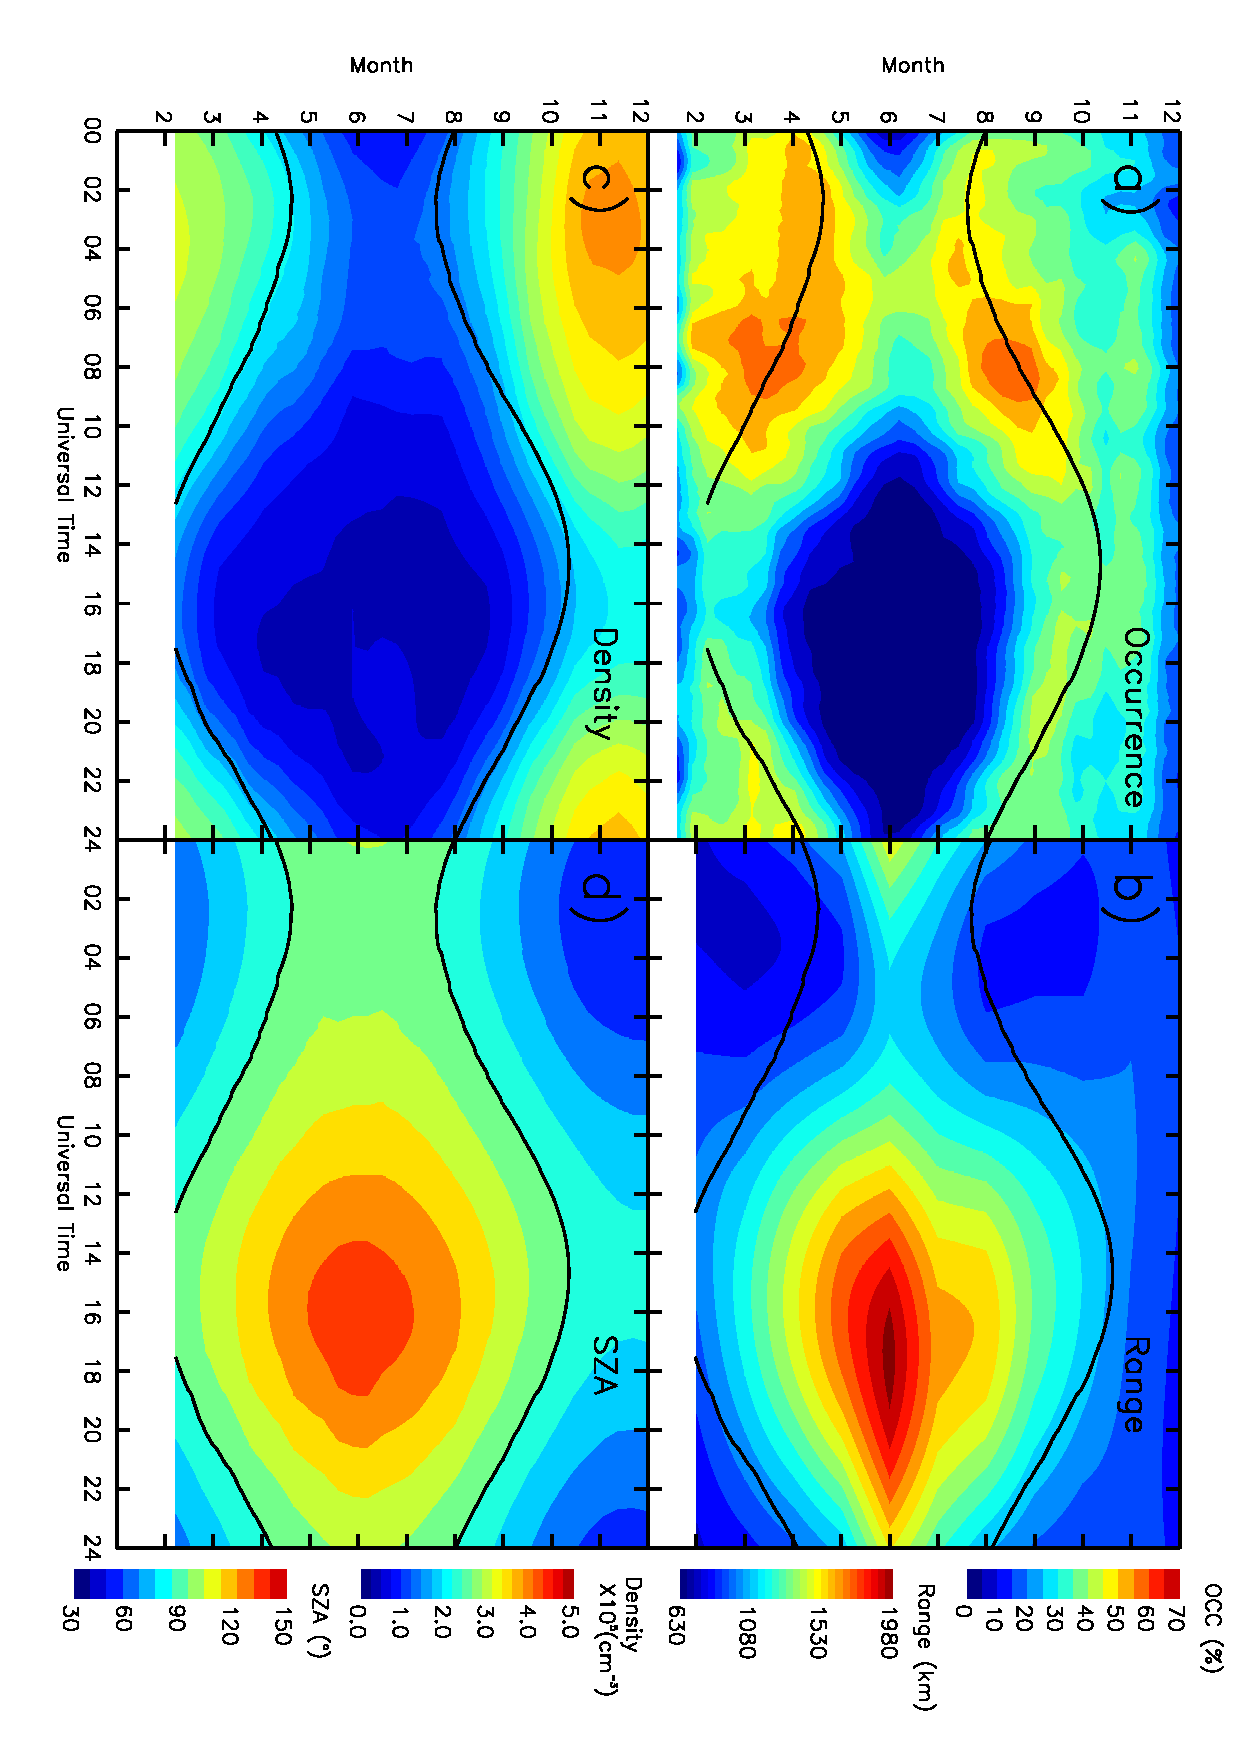
\includegraphics[width=12.0 cm,angle=90]{month_ut_combined2010.pdf}
\caption{Contour plots of the (a) average occurrence within the band, (b) band range, (c) model peak F-region electron density (NmF2) and (d) solar zenith angle (SZA) versus UT and month in 2010. Color bars are given to the right. The white rectangle at the bottom of each panel is due to no data available in January 2010.}
\label{fig:month_ut}
\end{figure}

A different view of occurrence dependencies on NmF2, SZA, and NmE was offered in Figure \ref{fig:scatter} in a more explicit form. The range and occurrence dependencies were found to be quite different, which, as discussed above, indicates that propagation effects are not dominant in occurrence variations. This is in contrast with the previous study by \citet{Kane2012} that conducted separate analyses for night- and daytime observations. The current approach resulted in a single and well-defined pattern that has a clear occurrence peak near a SZA of 90\(\deg\), i.e. near the solar terminator. This is also in contrast with previous studies where a qualitative agreement was observed between contours of constant occurrence and SZA \citep{Kane2012,Ghezelbash2014b}. Occurrence decreases on both sides of SZA of 90\(\deg\) but most likely for different reasons.

A decrease at smaller SZA is consistent with the idea of sunlight wiping out gradients necessary for GDI to operate. Increase in NmE resulting in shorting of \(F\) region irregularities by the conducting \(E\) layer may have also contributed. A decrease at larger SZA, on the other hand, is associated with a decreasing NmF2, increasing range, and stronger under-refraction effects. Importantly, however, not all of this decrease is due to stronger under-refraction. This is because range was increasing, but still well within the radar's FoV, Figure \ref{fig:scatter}a. That is, at the ranges where echoes were expected based on range trends, echoes were present but reduced in occurrence, Figure \ref{fig:month_avg_occ}a and c. Thus an alternative explanation must be sought for an occurrence decrease at large SZA. This could be due the scattering cross-section being effectively proportional to the square of background density, a plasma-physical effect described by \citet{Makarevich2014b}. In addition, the role of gradients near the solar terminator will also diminish.

A clear occurrence peak near the solar terminator is a strong indication of importance of large-scale gradients in production of small-scale irregularities. A traditional way of thinking about this disparity between scales is in terms of turbulent cascade from large-scale structures to smaller irregularities \citep{Tsunoda1988}. In this process, large-scale structures can become unstable due to GDI and other structuring mechanisms and act as seeds for smaller-scale structures. The current observations thus indicate that large-scale density gradients associated with the solar terminator can be a significant source of seeding structures.

\subsection{Irregularity Production in the IMF-Controlled Convection Environment}

The current study has also presented the first investigation of indirect solar effects due to IMF variations on irregularity production in the polar cap. It is well established that IMF variations directly control many high-latitude phenomena including auroral electrojets \citep[e.g.][]{McPherron1988}, plasma convection patterns \citep{Heelis1984,Ruohoniemi1996,Ridley1998,Pettigrew2010} and occurrence of optical auroras \citep{Ostgaard2004}. In contrast, only two studies have investigated IMF control of small-scale irregularity production and these focused on observations in the auroral \(F\) region \citep{Ballatore2001} and auroral \(E\) region \citep{Makarevich2012}.

This study found no clear evidence on such a control in the dayside polar cap, Figures \ref{fig:ut_occ} and \ref{fig:by_bz}. On the nightside (12--24 UT), however, a clear pattern emerged where echo occurrence was enhanced for negative IMF By and Bz, Figure \ref{fig:ut_occ}. The pattern for IMF Bx was nearly an inversion of that for IMF By, implying a high degree of correlation between IMF By and \(-\)Bx. Interestingly, however, the IMF Bz pattern was somewhat different from that of IMF By, Figure \ref{fig:ut_occ}, and in fact less clearly defined. Nevertheless, occurrence was generally higher for more negative IMF Bz, Figure \ref{fig:ut_occ}c. This result is consistent with the study by \citet{Ballatore2001} that also found higher occurrence for negative IMF Bz in the auroral zone. The new and unexpected result of the current study was that IMF By effects were more clearly defined in the occurrence of backscatter from the polar cap. Another new result of the current study was that the occurrence dependence on IMF was changing in a systematic way with UT on the nightside, Figures \ref{fig:ut_occ} and \ref{fig:by_bz}. For example, near 12 UT occurrence was generally above 80\% when IMF By was on average below \(-\)1.5 nT (blue cells at the top of Figure \ref{fig:ut_occ}b). On the other hand, for the same IMF By, but at a later UT, occurrence was between 60\% and 100\%, i.e. blue area of the plot expanded lower in Figure \ref{fig:ut_occ}b.

The echo occurrence dependence on IMF in general can be interpreted in context of IMF-controlled convection environment. High-latitude convection patterns are directly controlled by solar wind variations. Statistical convection patterns are derived from satellites and radars and are routinely parameterized by IMF By and Bz \citep{Haaland2007, Pettigrew2010}. One mechanism through which IMF-controlled variations in convection may be responsible for changes in occurrence of plasma irregularities involves changing orientations between plasma density gradients \(\vec{G}\) and convection velocity \(\vec{V}_E\) vectors. GDI can more easily excite waves when a component \(\vec{G}\cdot\vec{V}_E\) is more positive, with \(\vec{G}\parallel\vec{V}_E\) being most favorable orientation \citep{Keskinen1982a,Makarevich2014c}. IMF-controlled changes in \(\vec{V}_E\) can thus potentially lead to changes in \(\vec{G}\cdot\vec{V}_E\), which, in turn, will change GDI growth rate and occurrence of GDI-produced irregularities. This is a feasible basic scenario, although some questions still remain as to the extent of its contribution to the trends observed and reported here. For example, gradient scales must be relatively small for GDI to contribute to decameter-scale irregularity generation, with one widely-accepted possibility of large-scale gradient structures serving as seeds for small-scale structuring processes \citep{Tsunoda1988}. In this context, the presented results suggest that time scales at which convection changes are shorter than those associated with breakup of large-scale structures and changes in prevalent gradient orientations at both large and small spatial scales. This is consistent with the idea of very fast propagation of convection disturbances \citep{Ridley1998,Ruohoniemi2002,Fiori2012,Taguchi2015}.


\section{Summary and Conclusions}

Statistical analysis of backscatter from small-scale plasma irregularities observed by the SuperDARN McMurdo radar in the southern polar cap indicate that solar control of small-scale irregularity production in the polar cap is strong, multifaceted, and not restricted to the dayside. It exists in the form of (1) direct effects of local solar ionization that produce density gradients near the solar terminator and wipe out gradients on the dayside, (2) dayside ionization transported to the nightside as polar patches that routinely improve propagation conditions, and (3) solar wind variations that are responsible for changes in plasma convection and density gradient environment. Other important findings are as follows.

1. Backscatter location can be described reasonably well by using a simple model involving a cosine fit to diurnal variation in echo band position. The derived fit characteristics of the echo band display a clear pattern of diurnal, seasonal, and solar cycle changes that is very similar to those of the solar zenith angle and model peak \(F\) region density. The band range position is, therefore, strongly controlled by the local solar illumination conditions in the polar cap. On the nightside, however, a comparison between observations and model raytracing simulations reveal a presence of significant additional source of ionization. Conjugate observations of backscatter and density indicate that polar patches transported from the dayside are a viable source for this ionization.

2. Backscatter occurrence statistic exhibits evidence of both suppression and enhancement by sunlight, with a clear occurrence peak observed near the solar terminator. Suppression occurs at the largest SZA values observed and is consistent with diminishing role of gradients in irregularity production and increasing role of conducting $E$ layer. Enhancement by sunlight is mostly associated with more favorable propagation conditions at intermediate SZA values and large-scale gradients near the solar terminator possibly serving as seeds for further structuring processes.

3. Indirect control by the solar wind variations is limited to the nightside, with enhanced backscatter occurrence observed during intervals of negative IMF By and Bz. The IMF control of small-scale irregularity production can occur through IMF-controlled variations in the high-latitude convection pattern that, in turn, lead to changes in mutual orientations between convection and prevalent gradient vectors, with plasma structuring favoring certain orientations.



%\acknowledgments This work was supported by NSF grants AGS-1248127 and AGS-1341902. SuperDARN data are freely available through the SuperDARN website at Virginia Polytechnic Institute and State University http://vt.superdarn.org/. Fortran source code for IRI 2007 is freely available for download from the Community Coordinated Modeling Center (CCMC) at http://ccmc.gsfc.nasa.gov/. OMNI data is available from NASA Goddard Space Flight Center Space Physics Data Facility at http://omniweb.gsfc.nasa.gov. The Resolute Bay incoherent scatter radar (North) is operated by SRI International on behalf of the US National Science Foundation under NSF Cooperative Agreement AGS-1133009. The data are accessible from the SRI International online database at http://amisr.sri.com/database/. The authors thank W. A. Bristow for useful suggestions and providing the original Fortran source code for raytracing simulations. The developed IDL raytracing code is available from the corresponding author.




%\newpage
\bibliographystyle{uafthesis}
\bibliography{references}












%\end{article}
%\end{document}

%3 points:

%Solar control of irregularity production is not restricted to dayside
%Production peak near solar terminator implies breakup of large-scale structures
%Importance of IMF-controlled convection orientations relative to gradients



